\fancyhead[LO, RE]{Mettre en forme le texte}

\section{Mettre en forme la transcription}
\subsection{Pourquoi mettre en forme la transcription}
Après avoir récupéré la version océrisée des chapitres que nous étudierons par la suite, un premier nettoyage visuel a été fait, pour que l'information du fichier texte corresponde à ce qu'il y a dans le manuscrit et donc pour corriger les possibles erreurs qui sont apparues lors de la transformation du chapitre en une version texte. Une fois cela effectué, nous avons donc un fichier texte qui ressemble trait pour trait à la structure dans les différentes pages du manuscrit, ce qui permet ainsi d'avoir un document conforme si nous souhaitons simplement faire une reproduction exacte du manuscrit en version texte à étudier tel quel.

Cependant, pour la plupart des analyses et recherches à faire sur les chapitres du Beccaria, la forme du texte ne nous intéresse pas. L'analyse tend à se porter plutôt sur le fond, puisque le but du projet est de créer un dictionnaire de mots du droit et ainsi donc, étudier le contenu du texte et les mots utilisés. Dans un objectif plus proche, nous voulons principalement faire de l'alignement\index{Alignement} avec les différents chapitres, pour voir les changements (remplacements, insertions, suppressions) que les multiples éditeurs ont pu effectuer, et si certains de ces changements peuvent être une coupure de phrase ou un déplacement de paragraphes (pertinent pour notre analyse), d'autres éléments du texte ne nous intéressent pas et pourraient même fausser notre analyse. Nous entreprenons alors de mettre en forme le texte en écrivant un script Python qui sera adapté à toutes les versions du Beccaria et à toutes les éditions des chapitres, pour nettoyer et ménager un maximum d'informations.

\subsection{Réflexions sur les éléments à mettre en forme}
Il est nécessaire ensuite de s'interroger sur les éléments à traiter pour les voir disparaître ou changer et ainsi, faciliter au maximum notre analyse pour la suite du travail.

Le point le plus important à traiter était celui des coupures de mots. En effet, les manuscrits de l'époque n'offrant pas de très longs espaces pour écrire les textes, il y a de nombreux mots séparés par un tiret et une mise à la ligne. Ceux-ci représentent la correction la plus importante, puisque la méthode ou la taille d'écriture, la place allouée pour un chapitre ou l'espace de la feuille n'étaient pas toujours les mêmes en fonction du manuscrit et donc ce ne sont jamais les mêmes mots qui sont séparés en fonction des textes, mais lors des diverses analyses, ces mots sont considérés comme des différences entre deux versions ou ne sont pas comptés dans une analyse de correspondances, ce qui représente donc une grande marge d'erreur pour l'étude des texte.

Ensuite, de la même manière qu'avec les mots coupés par un tiret, le texte est segmenté en de très courtes lignes, qui ne permettent pas d'apprécier complètement les blocs de texte qui peuvent être similaires entre deux versions et il était donc nécessaire de faire également disparaître ces sauts de lignes, pour créer des paragraphes plus compacts. Un problème se pose cependant à ce stade de la réflexion, puisque nous ne souhaitons pas voir disparaître tous les sauts de lignes. Beccaria a décidé, lorsqu'il a rédigé son texte, de faire des séparations de paragraphes qui expriment sa pensée et sa manière de réfléchir. Cela a été repris par les éditeurs ou changé par d'autres, mais dans les deux cas, la place des paragraphes a une importance pour l'analyse du texte et nous allons donc chercher à conserver ces séparations, qui seront utiles notamment lors de la procédure d'alignement\index{Alignement}, pour réaliser un alignement\index{Alignement} par paragraphe. Il y a donc deux manières différentes d'appréhender la séparation du texte dans le script Python, ce qui a causé une certaine difficulté, comme cela s'observera par la suite.

Le troisième point auquel nous avons réfléchi était l'idée de supprimer des éléments plus mineurs qui auraient pu gêner dans l'analyse textuelle, tels que les majuscules, certains signes de ponctuations ou encore quelques symboles à régulariser. Après avis des membres du projet et notamment des linguistes, nous avons conclu de les garder, car cela n'empiétait pas sur l'analyse que nous effectuerons. Le seul élément mineur que nous avons décidé de supprimer est le numéro des pages présent pour montrer exactement la disposition dans le manuscrit~: l'élément nuit à la bonne lecture de notre document et n'est plus nécessaire avec la nouvelle mise en forme apportée au texte. Ainsi, le cahier des charges du script de mise en forme est établi et nous pouvons passer à la rédaction.

\subsection{Représentation de la mise en forme des transcription}
\begin{figure}[p]
    \centering
    \fbox{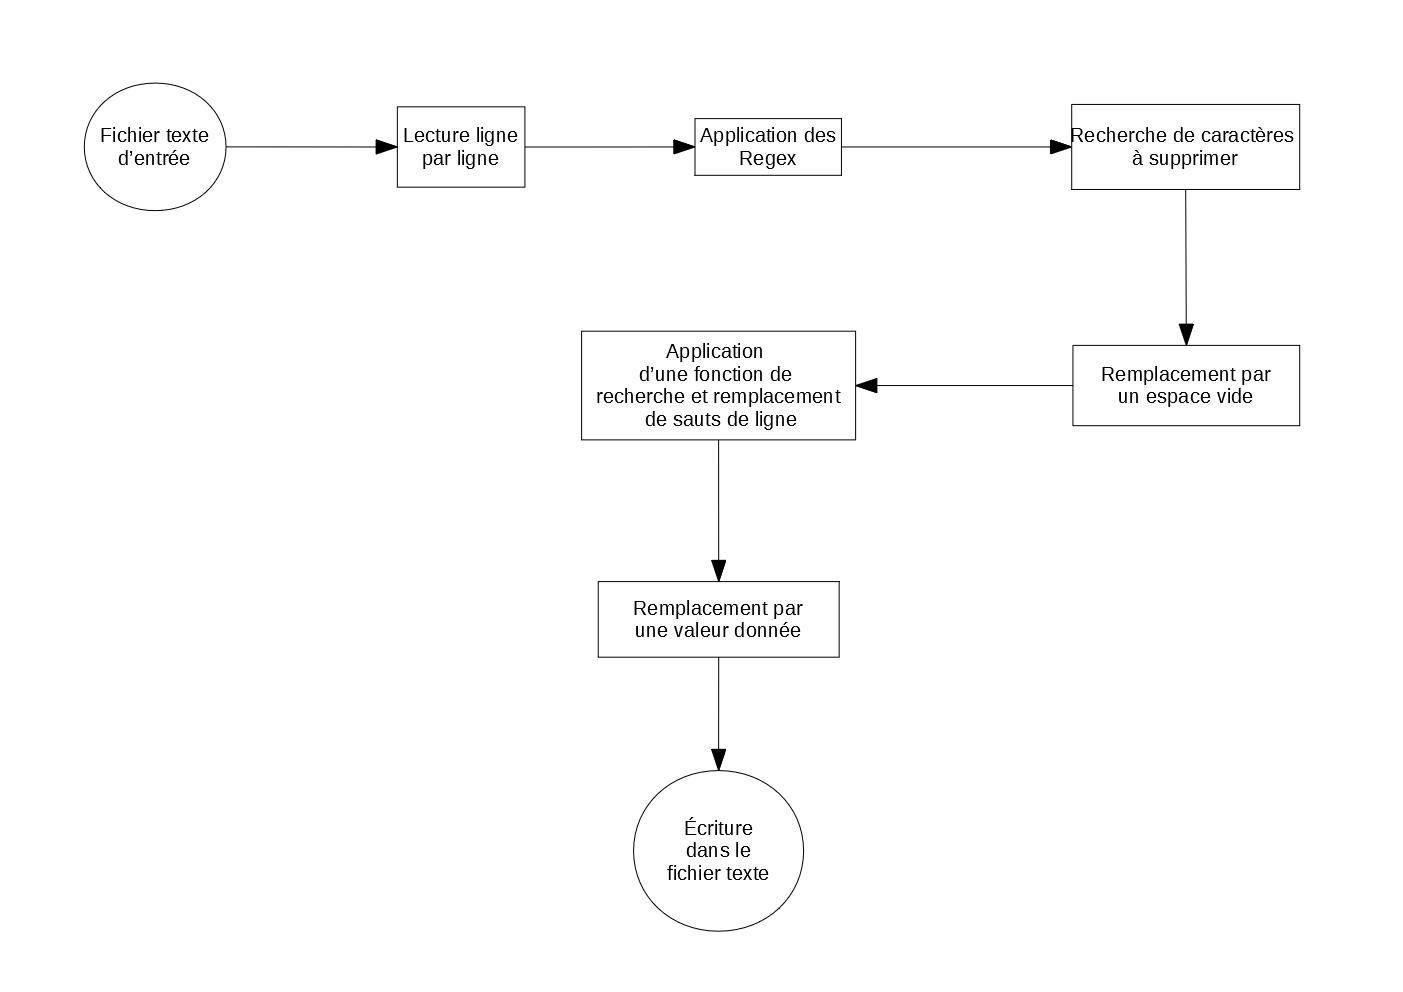
\includegraphics[width=14cm]{Partie2/schemas/3_mise_en_forme_bis.jpg}}
    \caption{Diagramme d'activité représentant les étapes pour mettre en forme les fichiers texte de transcription}
    \label{fig:etape3}
\end{figure}
Le diagramme d'activité de la figure \ref{fig:etape3} présente un traitement qui a pour objectif de partir d'un fichier d'entrée, soit la transcription directe du manuscrit pour arriver à un fichier de sortie qui sera la mise en forme souhaitée de ce texte. Ce processus lit le texte ligne par ligne pour trouver les éléments qu'il devra corriger. Il effectue ensuite deux tâches, il va tout d'abord, à l'aide d'expressions régulières, supprimer certains éléments du texte définis plus tôt, soit les numéros de pages et les tirets en fin de ligne, pour les remplacer par un simple espace. Ensuite, à l'aide d'une fonction de recherche et remplacement de sauts de ligne, ce traitement supprime les sauts de ligne inutiles tout en conservant les sauts de ligne qui correspondent à la fin d'un paragraphe et au début d'un autre. Une fois cela effectuée, la version mise en forme du texte est intégrée dans un fichier texte de sortie.
\begin{figure}[p]
    \centering
    \fbox{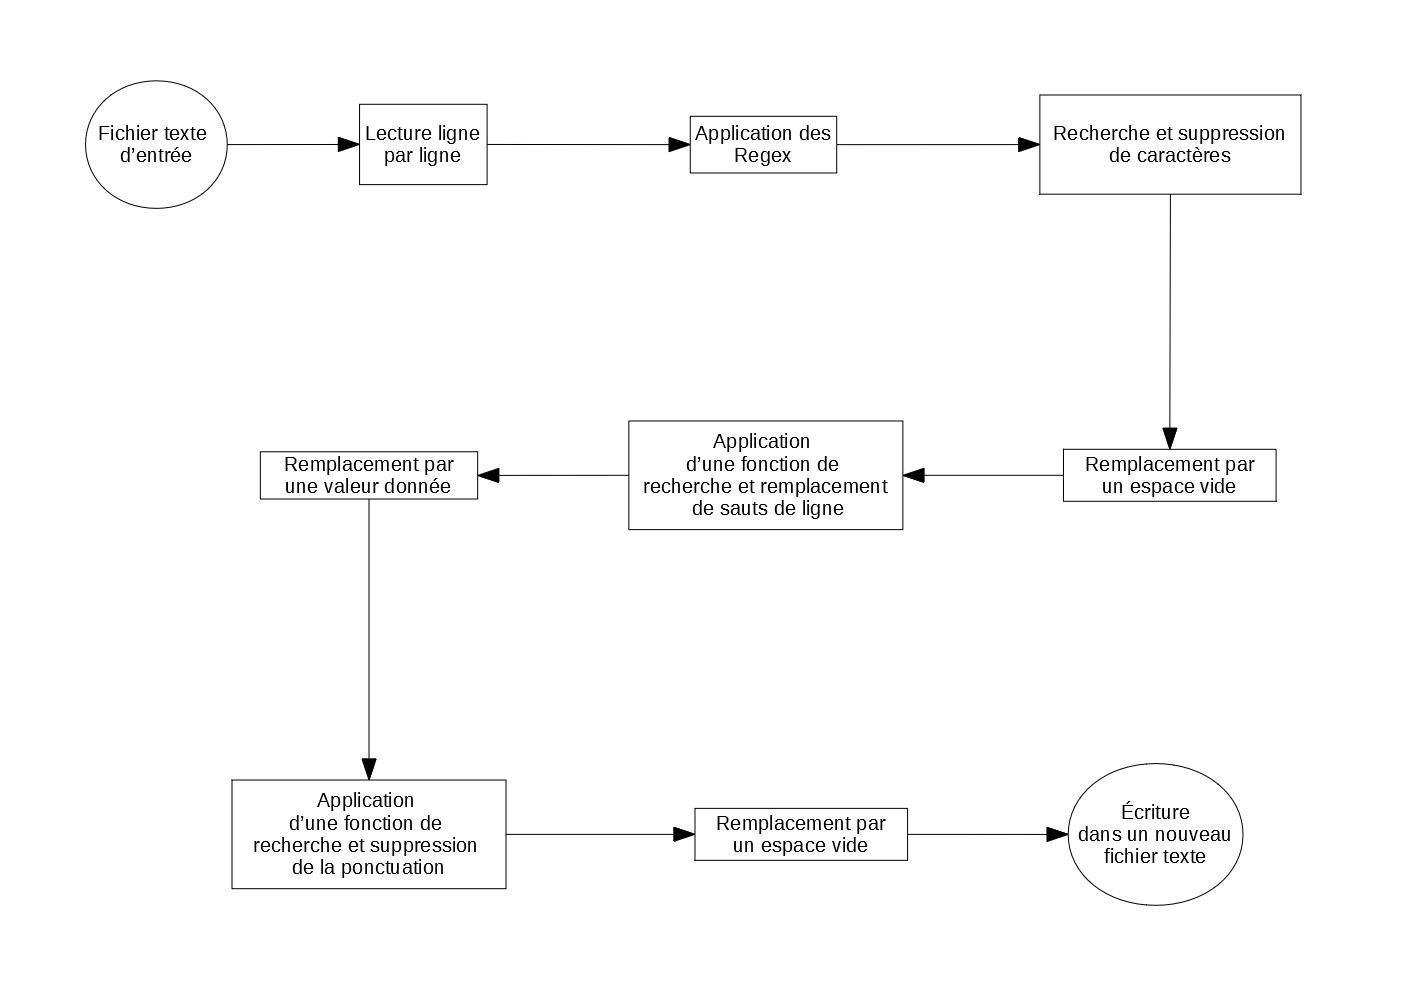
\includegraphics[width=14cm]{Partie2/schemas/1_mise_en_forme.jpg}}
    \caption{Diagramme d'activité représentant les étapes pour mettre en forme la transcription texte ainsi que supprimer des éléments de ponctuation.}
    \label{fig:etape1}
\end{figure}
Il y a dans le diagramme de la figure \ref{fig:etape1} les mêmes éléments qu'observés dans la figure \ref{fig:etape3}, mais une étape ici a été rajouté, celle de supprimer la ponctuation, ce qui sera nécessaire pour faciliter le travail du vérificateur orthographique, qui sera utilisé lors de la prochaine démarche. Nous incluons donc seulement cette étape avant de réaliser la vérification orthographique. Le fichier texte de mise en forme standard qui sera utilisé par la suite sera fait en suivant les étapes du diagramme d'activité de la figure \ref{fig:etape3}.

\section{Implémentation du script Python}
\subsection{Ajout des modules}
Nous avons commencé à réfléchir aux modules sur lesquels s'appuyer pour la rédaction et avons décidé d'utiliser majoritairement le module \emph{re} de Python. Il a pour but d'utiliser les expressions régulières, adéquat puisque notre démarche consiste à effectuer des remplacements au sein du texte. Nous avons également choisi d'utiliser le module \emph{sys} présent notamment dans les scripts d'\acrshort{ocr}\index{OCR} pour permettre de faire appel par la suite au script et aux paramètres qui seront donnés dans l'interpréteur de commande pour ainsi réaliser l'opération plus rapidement et plus efficacement. 

\subsection{Paramètres d'entrée et de sortie des fichiers}
Nous avons créé le script en premier lieu en définissant des paramètres qui ne concerneraient qu'un fichier unique, pour pouvoir tester rapidement sur un seul fichier si le script fonctionnait. Nous avons donc défini un fichier d'entrée en mode lecture et en encodage UTF-8 et un fichier de sortie en mode écriture, auxquels nous avons attribué une place pour la requête avec le terminal au moyen des \emph{sys.argv[]}. Par la suite, ces informations-là ont été retirées lorsque le script a été défini pour gérer un dossier complet de transcriptions et non juste un seul fichier. Nous avons alors importé le module \emph{os}, qui permet de manipuler des chemins pour aller chercher les fichiers qui nous intéressent dans un dossier. Nous avons ainsi inséré la fonction \emph{os.walk()} à laquelle a été ajouté un argument qui sera appelé dans la commande du terminal et qui correspondra au dossier contenant les transcriptions à normaliser. Nous avons ensuite redéfini les \emph{file\_in} et \emph{file\_out} pour qu'ils répondent à nos attentes et notamment que le fichier de sortie contienne une indication qui démontre que le document a été normalisé (\emph{sys.argv[2] + \og~/Norm~\fg{} + filename}). En fin de script, deux lignes de code permettent de fermer les deux fichiers et de clore le script.

\subsection{Boucler sur les lignes}
Après avoir paramétré le script, nous avons dû trouver un moyen de créer une boucle pour pouvoir travailler sur les lignes de texte pour effectuer les modifications nécessaires, étape observée au tout début du schéma de la figure \ref{fig:etape3}. Cette étape a donné lieu à de nombreux essais infructueux, pour trouver la technique la plus adéquate pour avoir correctement accès au contenu de notre texte. 
Notre premier essai était celui-ci~: 
\begin{minted}{python}
    for line in file_in:
\end{minted}
Nous nous sommes cependant vite rendu compte qu'une technique pareille prenait en compte le document ligne par ligne mais en les considérant comme de simples éléments détachés les uns des autres sans aucun lien, bloquant ainsi la majorité des manipulations effectuées dans le codage et n'apportant ainsi rien à notre mise en forme.

Nous avons alors tenté de trouver une manière de lire le document en plusieurs lignes liées entre elles, en utilisant plusieurs méthodes~:
\begin{itemize}
    \item \mint{python}{split_lines = line.splitlines()}
    \item \mint{python}{liste = [item for item in line.split('\n')]}
    \item \mint{python}{alltext = ' '.join(liste)}
    \item \mint{python}{for match in test.finditer(line):}
    \begin{itemize}
        \item \mint{python}{print(match.groups())}
    \end{itemize}
\end{itemize}
Cela ne correspondait jamais à ce que nous souhaitions faire ou ne donnait pas les résultats voulus pour la mise en forme. Nous avons finalement trouvé une méthode Python qui est dédiée à la lecture de lignes et notamment de plusieurs lignes (soit le texte en son entier), \emph{.readlines()}, défini ainsi par Python~:
\begin{quotation}
\og~\emph{f.readline()} lit une seule ligne du fichier~; un caractère de fin de ligne (\textbackslash n) est laissé à la fin de la chaîne. Il n'est omis que sur la dernière ligne du fichier si celui-ci ne se termine pas un caractère de fin de ligne. [...] Pour construire une liste avec toutes les lignes d'un fichier, il est aussi possible d'utiliser \emph{list(f)} ou \emph{f.readlines()}.\fg{} \footnote{Documentation Python~: 7 - Les entrées/sorties - \url{https://docs.python.org/fr/3/tutorial/inputoutput.html}}
\end{quotation}
Ainsi, avec cette méthode, le script va lire et analyser aisément les lignes, en prenant en compte certaines des informations précédant et suivant une ligne en particulier et ainsi, répondre aux attentes imposées lors de la recherche d'éléments dans le texte.

\subsection{Comment conserver la structure des paragraphes~: trouver la bonne expression régulière}
Comme cela a pu s'observer lors de la réflexion sur le script, nous voulons insérer plusieurs types d'éléments dans le code qui demandera plus ou moins de réflexions. La plupart des morceaux ne posent aucun problème, l'expression régulière correspondante n'étant pas trop difficile à trouver mais un cas en particulier pour la mise en forme a été assez ardu~: la structuration des paragraphes.

La transcription du manuscrit contenait deux types de cas pour lesquels devait s'appliquer une solution différente en fonction du cas, ce qui se présentait ainsi~:
\begin{itemize}
    \item Cas 1~: La phrase a été coupée en plein milieu et le saut de ligne doit disparaître, soit  \og~minuscule - saut de ligne - minuscule~\fg{} --> Changement en espace simple~;
    \item Cas 2~: La phrase finit par un point et est suivie d'un saut de ligne et la ligne suivante commence par une majuscule et cela doit être conservé, soit  \og~point  - saut de ligne - Début de mot avec une majuscule~\fg{} --> Conserver la mise à la ligne.
\end{itemize}
L'opération pour réaliser le cas 1 était plutôt simple puisqu'il suffisait juste de faire disparaître tous les sauts de lignes, mais dans ce cas, la structure du cas 2 est perdue. Nous avons alors cherché plusieurs types d'expressions régulières, qui répondraient à notre objectif, comme notamment signifier le cas 2 en expression régulière ( \og~.\textbackslash n[A-Z][A-Za-z] ~\fg{}) et lui dire que nous voulons conserver ce saut de ligne ou chercher à faire disparaître les sauts de ligne qui n'existent que pour le cas 1 ( \og~(.+)\textbackslash n(.+) ~\fg{}), ce qui n'a jamais donné aucun résultat concluant pour notre mise en forme.

Finalement, après réflexion, nous avons trouvé une solution mais elle implique d'effectuer trois étapes successives pour que l'objectif soit atteint et bien que le texte ne soit pas parfait ensuite, il répond au moins aux attentes pour la structure des pages.

Voilà comment se décompose la solution~:
\begin{itemize}
    \item Étape 1~: Modification du cas 2 en changeant le point de fin de phrase par un autre signe quelconque mais qui ne figure préférablement pas non plus dans le texte~;
    \item Étape 2~: Suppression de tous les sauts de ligne présents dans le texte pour obtenir un bloc compact du texte sans autre délimitation que les phrases~;
    \item Étape 3~: Réintégration des sauts de ligne là où il y a le signe de l'étape 1 et en même temps, remplacement de ce signe par le point d'origine.
\end{itemize}
Par conséquent, le texte retrouve la structuration de paragraphes que nous voulons conserver. Cependant, cette technique représente tout de même trois lignes de code pour une étape non trouvée avec une seule ligne et pour simplifier le code et permettre plus de clarté, ces étapes sont intégrées dans une fonction.

\subsection{Création des fonctions}
Si le script ne se compose pas d'un très grand nombre d'éléments, il existe certaines requêtes dans le codage qui nécessitent plus de deux à quatre lignes, ce qui peut faire lourd dans le code et notamment dans la boucle. Nous aurons alors recours à des fonctions pour donner un nom à ces étapes un peu longues et ainsi faciliter la lecture du code. Il y a deux fonctions plus ou moins complexes dans le script, dont une qui ne sera utilisée que partiellement.

\subsubsection{supprimer\_ponctuation()}
Pour mettre en forme le texte en suivant les instructions des responsables du projet, seuls les tirets et sauts de ligne, ainsi que numéros de page, doivent être supprimés. Nous ne devrons donc pas supprimer la ponctuation, nécessaire à une bonne compréhension du texte et à un souci d'authenticité vis-à-vis des auteurs ou traducteurs. En l'état, dans la version définitive du texte produite avec sa nouvelle mise en forme, la ponctuation est conservée. Cependant, une des étapes qui viendra après nécessite que la ponctuation soit supprimé et nous écrivons donc une fonction pour réaliser cela, fonction qui apparaît dans la figure \ref{fig:etape1}. Pour réaliser cela, j'ai extrait une fonction étudiée pendant les cours de Python, qui définit les signes de ponctuation à retirer et à l'aide d'une boucle \emph{for}, ils sont remplacés par du vide. J'ai modifié quelque peu le contenu de la variable ponctuation et j'y ai fait apparaître les différentes variantes de l'apostrophe ainsi que les points et j'ai retiré les tirets, car ils sont nécessaires à la compréhension de certains mots du texte. Une fois la fonction définie, elle est insérée dans les lignes de code de la boucle \emph{for} avec notre texte comme paramètre.

\subsubsection{mise\_a\_la\_ligne()}
Cette fonction reprend ce qui a été vu plus tôt dans notre réflexion pour conserver la structure du texte. Nous insérons donc dans cette fonction, à laquelle nous mettons comme paramètre un texte, les trois lignes de code pour conserver les paragraphes. Nous pouvons ensuite l'introduire dans notre boucle \emph{for} et limitons ainsi la longueur du code tout en ayant défini une fonction qui peut être réutilisée par la suite.

\section{Rédaction du script}
Le script est presque fait, tous les éléments nécessaires ont été définis et il faut maintenant écrire les lignes de code dans la boucle \emph{for} et nous suivons alors un certain cheminement pour entrer chaque ligne nécessaire pour le code.

Tout d'abord, les numérotations de pages sont supprimées car inutiles pour l'analyse du texte en lui-même. Ensuite, les mots séparés d'un tiret sont régularisés, car écrits ainsi pour le manuscrit et lors de l'océrisation\index{OCR!ocerisation@océrisation}, en supprimant le tiret et le saut à la ligne. Nous ajoutons également une variante, nécessaire pour les éditions allemandes, puisqu'il y a parfois le caractère  \og~=~\fg{} au lieu d'un tiret. Puis, une de nos fonctions est insérée, celle pour structurer les paragraphes. Enfin, la dernière fonction, définie dans le cas de l'utilisation du script pour la première étape de la vérification orthographique est appelée, soit la fonction pour supprimer les caractères de ponctuation à faire disparaître.

\section*{Conclusion~: application du script}
\addcontentsline{toc}{section}{Conclusion~: application du script}
Après application du script sur le chapitre utilisé comme exemple pour l'élaboration, nous pouvons observer le rendu. La structure du texte a été conservée, mais il y a néanmoins des coquilles. Certains mots n'ont pas été recollés correctement (du fait de leur séparation de base par un tiret et par le numéro de page) et beaucoup d'espaces non voulus sont également présents dans le texte, notamment au niveau des délimitations de paragraphes. La plupart de ces erreurs peuvent être corrigées par la suite à la main, sans que cela soit trop compliqué ou long, pour permettre ainsi d'avoir un texte répondant à toutes nos exigences pour l'analyse future.
Le script de mise en forme permet donc de présenter notre texte comme nous le souhaitions et nous pourrons, par la suite, l'appliquer aux chapitres suivants.